% Provenance (never printed): BCPST year 1 geology (2021), "la carte
% geologique" (reading a map, structures, chronology), union licence
% Sciences de la Terre L1 (cartographie: strike and dip, three-point problem,
% outcrop patterns, DEM and GIS). See sources/outline_sources.md. Pilot
% chapter, 2026-10-22. The region is the series' invented Varden Hills
% (figdata/shared/region.py); every number about it is computed in
% figdata/bachelor-1/varden_maps.py or figdata/bachelor-1/v_rule.py.
\chapter{地质图}\label{ch:b1:geological-maps}

一位地质学家带着图板、笔记本和
罗盘-测斜仪，穿过一片低矮的丘陵。大部分地面是草地、林地或已耕的田地；
岩石只在溪岸、公路切坡、岩崖等处零星露出。
根据这些零散的\omterm{def:b1:geological-maps:geological-map}{露头}以及地形的形状，地质学家必须判断
丘陵之下每平方米处是哪种岩石、岩层如何倾斜、
在何处断裂，以及这一切按何种顺序发生。
其成果是\omterm{def:b1:geological-maps:geological-map}{地质图}：一幅平面图，记录着一个三维的岩体。
本章说明这种图如何绘制、如何阅读——
包括面的\omterm{def:b1:geological-maps:attitude}{产状}如何测量和计算，为何层的\omterm{def:b1:geological-maps:geological-map}{露头}
描出那样的图案，以及地图如何记述历史。
本章的例子取自一个虚构但地质上自洽的地区，即
瓦尔登丘陵，它贯穿全书。

\begin{recall}
地形图用等高线表示地形起伏，等高线是高程相等的线；
其比例尺把图上距离与地面距离相联系
（第 1 册，九年级）。相对年代由叠加原理得出（一层岩层比其下的岩层年轻，
除非层序已经倒转），
由切割关系得出（切穿岩石的东西比该岩石年轻），并由
包含关系得出（第 1 册，七年级）。断层是两盘岩块
曾发生相对移动的断裂面（第 1 册，七年级）；\omterm{def:b1:geological-maps:fold}{褶皱}与断层的几何形态
在\cref{ch:b1:faults-folds-fabrics}中讨论。
\end{recall}

\section{地图是三维岩体的一个切面}\label{sec:b1:geological-maps:cut}

\begin{definition}[地质图]\label{def:b1:geological-maps:geological-map}
\emph{地质图}\index{地质图}给出地表每一点处土壤之下的岩石单元，
并给出\emph{地质界线}\index{地质界线}（分隔两个岩石单元的面），
以及影响它们的构造（断层、\omterm{def:b1:geological-maps:fold}{褶皱轴}、层的\omterm{def:b1:geological-maps:attitude}{产状}）。
\emph{填图单元}\index{填图单元}是一种可在野外识别和追踪的岩石体，
在图上用一种颜色绘出；
其\emph{露头}\index{露头}
即它在地表出露的区域。
\end{definition}

\begin{definition}[数字高程模型]\label{def:b1:geological-maps:dem}
\emph{数字高程模型}\index{数字高程模型}是地面高程的网格，
即在规则间隔的点上给出高程 $z = g(x,y)$。地理信息系统
存储这些网格以及地图的其他图层（\omterm{def:b1:geological-maps:geological-map}{地质界线}、
断层、测量数据、钻孔），并在共同的坐标框架中
进行计算。
\end{definition}

\begin{proposition}[地质界线的露头]\label{prop:b1:geological-maps:intersection}
设地面为曲面 $z = g(x,y)$，\omterm{def:b1:geological-maps:geological-map}{地质界线}为曲面
$z = c(x,y)$。\omterm{def:b1:geological-maps:geological-map}{地质界线}在图上的迹线是曲线
\[
  g(x,y) = c(x,y),
\]
即两曲面的交线在水平面上的投影，
位于界线之上的岩石单元在 $g > c$ 处出露。
\end{proposition}

\begin{proof}
图上一点位于迹线上，当且仅当该点处的地表落在界线上，
即 $g(x,y) = c(x,y)$。当
$g(x,y) > c(x,y)$ 时，地面位于界线之上：地表处的岩石
属于其上方的岩石单元。
\end{proof}

\begin{remark}[本书地图的绘制方法]\label{rem:b1:geological-maps:computed}
这正是地理信息系统从三维模型绘制地图的方式：
它在\omterm{def:b1:geological-maps:dem}{数字高程模型}的网格上计算 $g - c$，
并追踪其符号发生变化的曲线。本书中瓦尔登丘陵的地图
即按此方式绘制，所依据的地质模型中
每一个面都是已知的。
\end{remark}

\begin{omfigure}
\begin{tikzpicture}
\begin{axis}[axis equal image, xmin=0, xmax=10, ymin=0, ymax=8, width=0.82\linewidth,
  tick label style={font=\scriptsize}, xlabel={东 (km)}, ylabel={北 (km)},
  label style={font=\small}, colormap/blackwhite, enlargelimits=false]
\addplot[matrix plot*, mesh/cols=101, point meta=explicit, shader=interp] table[x=x_km, y=y_km, meta=shade] {figdata/out/bachelor-1-varden_maps-shade.dat};
\addplot[contour, line width=0.25pt, opacity=0.7] table {figdata/out/shared-region-contours.dat};
\addplot[index contour, opacity=0.8] table {figdata/out/shared-region-index-contours.dat};
\addplot[river] table {figdata/out/shared-region-river.dat};
\end{axis}
\end{tikzpicture}

{\small 瓦尔登丘陵的\omterm{def:b1:geological-maps:dem}{数字高程模型}：以西北方向光照的地面，
等高线每隔 \qty{50}{m} 一条（250 与
\qty{500}{m} 处加粗），河流向东流。}
\end{omfigure}

\begin{omfigure}
\begin{tikzpicture}
\begin{axis}[axis equal image, xmin=0, xmax=10, ymin=0, ymax=8, width=0.82\linewidth,
  tick label style={font=\scriptsize}, xlabel={东 (km)}, ylabel={北 (km)},
  label style={font=\small}]
\addplot[lith schist, draw=black, line width=0.3pt, even odd rule] table {figdata/out/shared-region-unit-schist.dat};
\addplot[lith granite, draw=black, line width=0.3pt, even odd rule] table {figdata/out/shared-region-unit-granite.dat};
\addplot[om lith={icsTriassic!35}{om sand}, draw=black, line width=0.3pt, even odd rule] table {figdata/out/shared-region-unit-sandstone.dat};
\addplot[om lith={icsJurassic!40}{om limestone}, draw=black, line width=0.3pt, even odd rule] table {figdata/out/shared-region-unit-limestone.dat};
\addplot[om lith={icsJurassic!15}{om shale}, draw=black, line width=0.3pt, even odd rule] table {figdata/out/shared-region-unit-shale.dat};
\addplot[om lith={icsCretaceous!35}{om limestone}, draw=black, line width=0.3pt, even odd rule] table {figdata/out/shared-region-unit-chalk.dat};
% the fault is drawn before the alluvium: the younger alluvial floor conceals it
\addplot[normal fault] table {figdata/out/shared-region-fault.dat};
\addplot[lith alluvium, draw=black, line width=0.3pt, even odd rule] table {figdata/out/shared-region-unit-alluvium.dat};
\addplot[contour, opacity=0.55] table {figdata/out/shared-region-contours.dat};
\addplot[river] table {figdata/out/shared-region-river.dat};
\pic at (axis cs:4.3,6.6) {strikedip={350.6}{12}};
\pic at (axis cs:2.2,6.6) {strikedip={189.3}{12}};
\pic at (axis cs:8.6,1.4) {northarrow};
\fill[black] (axis cs:6.6,0.35) rectangle (axis cs:7.1,0.5);
\fill[white] (axis cs:7.1,0.35) rectangle (axis cs:7.6,0.5);
\fill[black] (axis cs:7.6,0.35) rectangle (axis cs:8.1,0.5);
\fill[white] (axis cs:8.1,0.35) rectangle (axis cs:8.6,0.5);
\draw[black, line width=0.4pt] (axis cs:6.6,0.35) rectangle (axis cs:8.6,0.5);
\node[font=\footnotesize, above, inner sep=1.5pt, fill=white, fill opacity=0.8, text opacity=1] at (axis cs:7.6,0.5) {\qty{2}{km}};
\end{axis}
\end{tikzpicture}

\smallskip
\begin{tikzpicture}[font=\footnotesize]
\matrix[column sep=7pt, row sep=3pt, matrix of nodes, nodes={anchor=west}] {
  \tikz\draw[black!60, line width=0.4pt, lith alluvium] (0,0) rectangle (0.7,0.32); & 冲积层（第四纪） &
  \tikz\draw[black!60, line width=0.4pt, om lith={icsCretaceous!35}{om limestone}] (0,0) rectangle (0.7,0.32); & 白垩（白垩纪，90 Ma） \\
  \tikz\draw[black!60, line width=0.4pt, om lith={icsJurassic!15}{om shale}] (0,0) rectangle (0.7,0.32); & 页岩（侏罗纪，165 Ma） &
  \tikz\draw[black!60, line width=0.4pt, om lith={icsJurassic!40}{om limestone}] (0,0) rectangle (0.7,0.32); & 石灰岩（侏罗纪，180 Ma） \\
  \tikz\draw[black!60, line width=0.4pt, om lith={icsTriassic!35}{om sand}] (0,0) rectangle (0.7,0.32); & 砂岩（三叠纪，245 Ma） &
  \tikz\draw[black!60, line width=0.4pt, lith granite] (0,0) rectangle (0.7,0.32); & 花岗岩（310 Ma） \\
  \tikz\draw[black!60, line width=0.4pt, lith schist] (0,0) rectangle (0.7,0.32); & 片岩（480 Ma） &
  \tikz\draw[normal fault] (0,0.16) -- (0.9,0.16); & 正断层（刻线位于下降盘一侧） \\
};
\end{tikzpicture}

{\small 瓦尔登丘陵\omterm{def:b1:geological-maps:geological-map}{地质图}，包括等高线、河流、
两处实测\omterm{def:b1:geological-maps:attitude}{产状}（\omterm{def:b1:geological-maps:attitude}{走向}线与\omterm{def:b1:geological-maps:attitude}{倾向}刻线，并标注\omterm{def:b1:geological-maps:attitude}{倾角}度数）
以及图例。图中年龄为该区各单位的年龄；断层
隐伏于谷底较年轻的冲积层之下。}
\end{omfigure}

\section{平面的产状}

\begin{definition}[走向、倾角与倾向]\label{def:b1:geological-maps:attitude}
设地质面——层面、接触面、断层面——局部为
一平面。其\emph{走向}\index{走向}为所含水平线的方向，
以\omterm{def:b1:spherical-astronomy:horizontal}{方位角}表示（自北顺时针量起的度数）。
其\emph{倾角}\index{倾角} $\delta$ 为该平面与水平面之间的夹角，
在与走向垂直的竖直面内量取，
$0 \le \delta \le \ang{90}$。其\emph{倾向}\index{倾向}
$\alpha$ 为平面上最陡下倾直线的\omterm{def:b1:spherical-astronomy:horizontal}{方位角}。二者合称
平面的\emph{产状}\index{产状（平面）}，记作
倾向/倾角，例如 $080/12$。
\end{definition}

\begin{notation}[按右手定则确定走向]\label{not:b1:geological-maps:rhr}
同一\omterm{def:b1:geological-maps:attitude}{走向}可按两个相反方向读取。\emph{右手定则}
选取使得沿\omterm{def:b1:geological-maps:attitude}{走向}观察时平面向观察者右侧倾斜的那一个方向，即
\omterm{def:b1:geological-maps:attitude}{走向} $= \alpha - \ang{90}$（模 \ang{360}）。在地图上，
符号为一条\omterm{def:b1:geological-maps:attitude}{走向}线，带有一短刻线指向倾斜方向，
并标注\omterm{def:b1:geological-maps:attitude}{倾角}。
\end{notation}

\begin{omfigure}
\tdplotsetmaincoords{65}{125}
\begin{tikzpicture}[tdplot_main_coords, font=\small, scale=1.05]
  % the horizontal plane
  \fill[omSea!50] (-2.2,-1.6,0) -- (2.2,-1.6,0) -- (2.2,1.6,0) -- (-2.2,1.6,0) -- cycle;
  \draw[black!40] (-2.2,-1.6,0) -- (2.2,-1.6,0) -- (2.2,1.6,0) -- (-2.2,1.6,0) -- cycle;
  % the dipping plane: strike along y (north), dipping east (+x) at 30 degrees
  \fill[omLithLime!80, opacity=0.85] (-0.0,-1.6,0) -- (-0.0,1.6,0) -- (2.2,1.6,-1.27) -- (2.2,-1.6,-1.27) -- cycle;
  \draw[black!60] (0,-1.6,0) -- (0,1.6,0) -- (2.2,1.6,-1.27) -- (2.2,-1.6,-1.27) -- cycle;
  % strike line (horizontal, in both planes)
  \draw[omThm, line width=1.1pt] (0,-1.6,0) -- (0,1.6,0);
  % dip line and the horizontal below it, with the dip angle
  \draw[omDef, line width=1.1pt, -{Stealth[length=2.4mm]}] (0,0,0) -- (2.2,0,-1.27);
  \draw[black!60, densely dashed] (0,0,0) -- (2.2,0,0);
  \draw[black!60, densely dashed] (2.2,0,0) -- (2.2,0,-1.27);
  \draw[black] plot[domain=0:30, samples=16, variable=\t] ({0.8*cos(\t)}, 0, {-0.8*sin(\t)});
  \node[font=\footnotesize] at (1.05,0,-0.22) {$\delta$};
  % north arrow on the horizontal plane
  \draw[black, -{Stealth[length=2mm]}] (-1.8,-1.2,0) -- (-1.8,-0.3,0);
  \node[font=\footnotesize] at (-1.8,-0.05,0) {北};
\end{tikzpicture}
\begin{tikzpicture}[font=\small]
  \node[align=left, anchor=west, text width=5.2cm] at (0,0) {%
    \textcolor{omThm}{\rule[0.5ex]{0.6cm}{1.1pt}} 走向：平面内的一条水平线；\\[3pt]
    \textcolor{omDef}{\rule[0.5ex]{0.6cm}{1.1pt}} 平面上最陡的下倾直线，其方位角即倾向；\\[3pt]
    倾角为该直线与水平面（虚线）之间的夹角。};
\end{tikzpicture}

{\small \omterm{def:b1:geological-maps:attitude}{走向}为北、向东倾斜 \ang{30} 的平面（\omterm{def:b1:geological-maps:attitude}{产状}
$090/30$），沿其\omterm{def:b1:geological-maps:attitude}{走向}线切割水平面。未按比例绘制。}
\end{omfigure}

\begin{proposition}[倾斜平面的方程]\label{prop:b1:geological-maps:plane}
取 $x$ 指向东，$y$ 指向北，$z$ 竖直向上，
则\omterm{def:b1:geological-maps:attitude}{倾向}为 $\alpha$、\omterm{def:b1:geological-maps:attitude}{倾角}为 $\delta$、过点 $(x_0, y_0, z_0)$ 的平面为
\[
  z = z_0 - \tan\delta\,\bigl[(x - x_0)\sin\alpha + (y - y_0)\cos\alpha\bigr].
\]
\end{proposition}

\begin{proof}
沿\omterm{def:b1:geological-maps:attitude}{倾向}方向的水平单位向量为
$\vec u = (\sin\alpha, \cos\alpha, 0)$（\omterm{def:b1:spherical-astronomy:horizontal}{方位角}自北量起，
即自 $y$ 轴（北）向 $x$ 轴（东）量取）。沿\omterm{def:b1:geological-maps:attitude}{走向}，即与
$\vec u$ 垂直的方向，平面为水平的；沿 $\vec u$，每
单位水平距离下降 $\tan\delta$。点到过 $(x_0, y_0)$ 的
\omterm{def:b1:geological-maps:attitude}{走向}线的水平距离（沿\omterm{def:b1:geological-maps:attitude}{倾向}向下为正）为
$(x-x_0)\sin\alpha + (y-y_0)\cos\alpha$，由此得公式。
\end{proof}

\begin{theorem}[由三点确定产状]\label{thm:b1:geological-maps:three-point}
设 $P_1, P_2, P_3$ 为某平面上三个不共线的点，且
$\vec n = \overrightarrow{P_1P_2} \times \overrightarrow{P_1P_3} =
(n_x, n_y, n_z)$，取 $n_z > 0$（若不然，则将 $\vec n$ 换为 $-\vec n$
）。于是平面的\omterm{def:b1:geological-maps:attitude}{倾角}与\omterm{def:b1:geological-maps:attitude}{倾向}分别为
\[
  \delta = \arccos\frac{n_z}{\|\vec n\|}, \qquad
  \alpha = \text{ 水平向量的方位角 } (n_x, n_y),
\]
即角 $\alpha \in [\ang{0}, \ang{360})$，使得
$\sin\alpha = n_x/\sqrt{n_x^2+n_y^2}$ 与 $\cos\alpha = n_y/\sqrt{n_x^2+n_y^2}$
（若 $n_x = n_y = 0$，则平面水平）。
\end{theorem}

\begin{proof}
$\vec n$ 与平面内两个线性无关的向量垂直，故
它为平面的法向量。\omterm{def:b1:geological-maps:attitude}{倾角}即平面与水平面的夹角，
等于两法向量的夹角，即 $\vec n$ 与竖直向上的
$\vec k$ 之间的夹角，$\cos\delta = \vec n \cdot \vec k / \|\vec n\| = n_z/\|\vec n\|$。
由\cref{prop:b1:geological-maps:plane}可知，平面为 $z = \text{常数} -
\tan\delta\,(x\sin\alpha + y\cos\alpha)$，即
$\tan\delta\sin\alpha\,x + \tan\delta\cos\alpha\,y + z = \text{常数}$；其
向上的法向量与 $(\tan\delta\sin\alpha,
\tan\delta\cos\alpha, 1)$ 成比例，其水平分量指向
\omterm{def:b1:geological-maps:attitude}{倾向} $\alpha$ 方向。由于 $\vec n$ 为该法向量的正倍数，则 $(n_x, n_y)$
同样指向\omterm{def:b1:geological-maps:attitude}{倾向}。
\end{proof}

\begin{method}[三点问题]\label{met:b1:geological-maps:three-point}
求某一接触面在三个钻孔（或三处\omterm{def:b1:geological-maps:geological-map}{露头}）中
所见的\omterm{def:b1:geological-maps:attitude}{产状}：
\begin{enumerate}
  \item 对每个钻孔，取该接触面的高程：地面
        高程减去遇到接触面的深度；
  \item 以米为单位写出三点 $P_i = (x_i, y_i, z_i)$，$x$ 向东，
        $y$ 向北；
  \item 计算 $\vec n = \overrightarrow{P_1P_2} \times
        \overrightarrow{P_1P_3}$，并使 $n_z$ 为正；
  \item 应用\cref{thm:b1:geological-maps:three-point}，给出\omterm{def:b1:geological-maps:attitude}{产状}，
        以\omterm{def:b1:geological-maps:attitude}{倾向}/\omterm{def:b1:geological-maps:attitude}{倾角}表示；若需要，则由右手
        定则求出\omterm{def:b1:geological-maps:attitude}{走向}。
\end{enumerate}
在图纸上，同一问题可用构造等高线求解：在
最高点与最低点的连线上，按比例求出与
第三点等高的点；过这两点的直线即为
一条\omterm{def:b1:geological-maps:attitude}{走向}线；\omterm{def:b1:geological-maps:attitude}{倾角}则由两条平行\omterm{def:b1:geological-maps:attitude}{走向}线之间的
高程差及其间距求得。
\end{method}

\begin{example}[瓦尔登背斜的东翼]\label{ex:b1:geological-maps:east}
% computed in figdata/bachelor-1/varden_maps.py (boreholes E1-E3)
三个钻孔 E1 位于 $(4000, 6000)$，E2 位于 $(4600, 7200)$ 及 E3 位于
$(5100, 6400)$（以米计，为距图幅西南角的东向与北向距离），
它们遇到石灰岩底面的高程分别为 $174$、$4$ 和 $\qty{-74}{m}$。于是
$\overrightarrow{P_1P_2} = (600, 1200, -170)$，
$\overrightarrow{P_1P_3} = (1100, 400, -248)$；其叉积为
$(-229\,600, -38\,200, -1\,080\,000)$，指向下方，因此
\[
  \vec n = (229\,600,\ 38\,200,\ 1\,080\,000).
\]
由此可得 $\cos\delta = 1\,080\,000/\|\vec n\| \approx
0.9776$，$\delta \approx \ang{12.2}$，\omterm{def:b1:geological-maps:attitude}{倾向}即
$(229\,600, 38\,200)$ 的\omterm{def:b1:spherical-astronomy:horizontal}{方位角}，$\alpha \approx \ang{80.6}$。\omterm{def:b1:geological-maps:attitude}{产状}为
$081/12$，由右手定则得\omterm{def:b1:geological-maps:attitude}{走向} $\ang{351}$。石灰岩底面
向东北偏东缓倾。
\end{example}

\section{露头图样}

\begin{proposition}[水平与竖直接触面]\label{prop:b1:geological-maps:hv}
水平接触面的迹线沿其高程的等高线延伸。
竖直接触面的迹线在图上为一条直线，
与地形起伏无关。
\end{proposition}

\begin{proof}
对 $c(x,y) = z_0$，迹线 $g(x,y) = z_0$ 即等高线 $z_0$
（见\cref{prop:b1:geological-maps:intersection}）。竖直平面是水平位置
落在同一条直线上、任意高程的点的集合；
其在图上的迹线即该直线。
\end{proof}

\begin{theorem}[V 字法则]\label{thm:b1:geological-maps:v-rule}
一个平面状接触面穿过一条山谷，谷底沿下游方向
以坡度 $s > 0$ 下降。设 $a$ 为接触面在下游方向上的视\omterm{def:b1:geological-maps:attitude}{倾角}正切
（若向下游倾斜，则 $a > 0$；若向上游倾斜，则 $a < 0$；
若水平，则 $a = 0$）。于是\omterm{def:b1:geological-maps:geological-map}{露头}迹线呈 V 形，其顶点
位于谷底，且
\begin{itemize}
  \item 若 $a > s$，V 形指向\emph{下游}：接触面向下游倾斜的程度
        大于谷底下降的程度；
  \item 若 $a < s$，V 形指向\emph{上游}：接触面水平、向上游倾斜，
        或向下游倾斜但倾斜程度小于谷底。
\end{itemize}
竖直接触面不形成 V 形。
\end{theorem}

\begin{proof}
设 $\xi$ 为沿谷底向下游量取的距离。谷底
高程为 $z_g(\xi) = z_0 - s\xi$；在沿谷的竖直剖面中，
接触面位于 $z_c(\xi) = c - a\xi$。在谷底上，
迹线位于 $z_g = z_c$ 处：
\[
  \xi_{\text{谷底}} = \frac{c - z_0}{a - s}.
\]
在谷坡上，取比谷底高 $h > 0$、且与谷源距离相同的点，
地面高程为 $z_0 - s\xi + h$，因此
迹线位于 $c - a\xi = z_0 - s\xi + h$ 处：
\[
  \xi_{\text{谷坡}} = \frac{c - z_0 - h}{a - s}, \qquad
  \xi_{\text{谷底}} - \xi_{\text{谷坡}} = \frac{h}{a - s}.
\]
若 $a > s$，迹线在谷底上比在谷坡上更靠下游：
V 形指向下游。若 $a < s$，则情况相反。竖直接触面
穿过谷底与谷坡时对应的 $\xi$ 相同。
\end{proof}

\begin{omfigure}
\begin{tikzpicture}
\pgfplotsset{vpanel/.style={axis equal image, xmin=-1, xmax=1, ymin=0, ymax=2,
  width=4.1cm, ticks=none, axis line style={black!50}, clip=true,
  title style={font=\footnotesize, align=center, yshift=-2pt}}}
\begin{axis}[vpanel, at={(0cm,0cm)}, title={水平}]
\addplot[contour, opacity=0.8] table {figdata/out/bachelor-1-v_rule-contours.dat};
\addplot[omThm, line width=1.2pt] table {figdata/out/bachelor-1-v_rule-h.dat};
\addplot[river, -{Stealth[length=1.6mm]}] coordinates {(0,0.05) (0,1.95)};
\end{axis}
\begin{axis}[vpanel, at={(3.15cm,0cm)}, title={向上游 \\倾斜}]
\addplot[contour, opacity=0.8] table {figdata/out/bachelor-1-v_rule-contours.dat};
\addplot[omThm, line width=1.2pt] table {figdata/out/bachelor-1-v_rule-u.dat};
\addplot[river, -{Stealth[length=1.6mm]}] coordinates {(0,0.05) (0,1.95)};
\end{axis}
\begin{axis}[vpanel, at={(6.3cm,0cm)}, title={向下游，\\倾斜较缓}]
\addplot[contour, opacity=0.8] table {figdata/out/bachelor-1-v_rule-contours.dat};
\addplot[omThm, line width=1.2pt] table {figdata/out/bachelor-1-v_rule-g.dat};
\addplot[river, -{Stealth[length=1.6mm]}] coordinates {(0,0.05) (0,1.95)};
\end{axis}
\begin{axis}[vpanel, at={(9.45cm,0cm)}, title={向下游，\\倾斜较陡}]
\addplot[contour, opacity=0.8] table {figdata/out/bachelor-1-v_rule-contours.dat};
\addplot[omThm, line width=1.2pt] table {figdata/out/bachelor-1-v_rule-d.dat};
\addplot[river, -{Stealth[length=1.6mm]}] coordinates {(0,0.05) (0,1.95)};
\end{axis}
\end{tikzpicture}

{\small 图中为计算得出的 V 形规则。每幅图中，一条河流（蓝色箭头）向北
沿山谷流下，山谷的等高线（每隔 \qty{10}{m}）指向上游；
一条\omterm{def:b1:geological-maps:attitude}{走向}东西的接触面以红色标出。水平时，它沿等高线延伸；
\omterm{def:b1:geological-maps:attitude}{倾向}上游，或\omterm{def:b1:geological-maps:attitude}{倾向}下游但比谷底平缓时，
形成指向上游的 V 形；\omterm{def:b1:geological-maps:attitude}{倾向}下游且比谷底陡（此处为 \ang{10}）时，
则形成指向下游的 V 形。直立的接触面则笔直穿过。}
\end{omfigure}

\begin{remark}[露头宽度]\label{rem:b1:geological-maps:width}
单元\omterm{def:b1:geological-maps:geological-map}{露头}的宽度取决于其厚度、\omterm{def:b1:geological-maps:attitude}{倾角}以及地面坡度：
一层薄层若与坡面\omterm{def:b1:geological-maps:attitude}{倾向}相同，可在较大范围内出露。
厚度可由地图与
剖面在\cref{ch:b1:cross-sections}中求得。
\end{remark}

\section{地图上的褶皱、断层、侵入体与不整合}

\begin{definition}[背斜与向斜]\label{def:b1:geological-maps:fold}
\emph{褶皱}\index{褶皱}是原为平面状岩层的弯曲。
\emph{背斜}\index{背斜}是岩层向上凸起（上拱）的褶皱；
\emph{向斜}\index{向斜}是岩层向上凹陷（下凹）的褶皱。
褶皱的两侧称为其翼；其
\emph{褶皱轴}\index{褶皱轴}是岩层弯曲最剧烈的连线，
轴线不水平时即发生倾伏。像褶皱轴这样的直线，
由其倾伏向（沿下倾方向量取的水平投影的\omterm{def:b1:spherical-astronomy:horizontal}{方位角}）
和倾伏角（与水平面所成的夹角）确定
（见\cref{ch:b1:field-lab-methods-1}）。三维的褶皱几何
是\cref{ch:b1:faults-folds-fabrics}的内容。
\end{definition}

\begin{proposition}[褶皱的图形特征]\label{prop:b1:geological-maps:folds}
在被侵蚀\omterm{def:b1:geological-maps:fold}{褶皱}岩层的\omterm{def:b1:geological-maps:geological-map}{地质图}上，\omterm{def:b1:geological-maps:fold}{背斜}显示最老的
单元位于其核部，两侧向外依次为较新的单元；\omterm{def:b1:geological-maps:fold}{向斜}显示最新的
单元位于其核部。若\omterm{def:b1:geological-maps:fold}{褶皱轴}倾伏，\omterm{def:b1:geological-maps:geological-map}{露头}线会在\omterm{def:b1:geological-maps:fold}{褶皱}周围闭合：\omterm{def:b1:geological-maps:fold}{背斜}的
闭合端指向倾伏方向，
\omterm{def:b1:geological-maps:fold}{向斜}的闭合端则指向相反方向。
\end{proposition}

\begin{proof}[部分证明]
在\omterm{def:b1:geological-maps:fold}{背斜}中，岩层向轴线抬升，因此近于水平的侵蚀面
在此处切入地层最深，暴露出最老、最下部的单元；
在\omterm{def:b1:geological-maps:fold}{向斜}中，最新的单元保存在最下部，即核部。
若\omterm{def:b1:geological-maps:fold}{褶皱轴}倾伏，考虑\omterm{def:b1:geological-maps:fold}{背斜}的一个接触面：它是一个拱形，
其顶脊沿倾伏方向下降。当顶脊高于地面时，地面沿两翼切割拱形；
当顶脊低于地面时，接触面不再到达地表。
因此，痕迹的两翼在顶脊与地面相交处汇合，这一闭合端
位于倾伏方向上。\omterm{def:b1:geological-maps:fold}{向斜}是一个槽形，其底部向相反方向抬升，
因此其闭合端与倾伏方向相反。
该论证假定地形起伏
相对于轴线的下降幅度较小。
\end{proof}

\begin{proposition}[断层、侵入体与不整合]\label{prop:b1:geological-maps:cuts}
在\omterm{def:b1:geological-maps:geological-map}{地质图}上：
\begin{itemize}
  \item 断层切断并错开其所穿过的接触面；在下降的一盘上，
        较新的单元与对侧较老的单元出露于地表；
        倾斜断层的迹线与任何平面一样遵循 V 形规则；
  \item 深成岩体或岩墙切穿其所侵入岩石的接触面，
        且比这些岩石年轻；
  \item 在不整合处，较老岩层的接触面
        被截断于较新岩层的底面，较新岩层
        可能依次覆盖在若干较老单元之上。
\end{itemize}
\end{proposition}

\begin{method}[从地质图读取历史]\label{met:b1:geological-maps:history}
\begin{enumerate}
  \item 按年代先后列出各单元，
        依据图例与叠加原理。
  \item 找出相互切割关系：断层、侵入体、不整合；每一者都
        比其所切断的一切都年轻，比封盖它的
        一切都古老。
  \item 找出\omterm{def:b1:geological-maps:fold}{褶皱}及其\omterm{def:b1:geological-maps:fold}{褶皱轴}；\omterm{def:b1:geological-maps:fold}{褶皱}比其所\omterm{def:b1:geological-maps:fold}{褶皱}的
        最新单元年轻。
  \item 按先后写出各事件，并注明地图上的证据。
\end{enumerate}
\end{method}

\begin{example}[瓦尔登丘陵的历史]\label{ex:b1:geological-maps:history}
在瓦尔登丘陵的地图上：片岩最老；花岗岩切穿它，故较新；
砂岩覆盖于两者之上，并截去花岗岩的轮廓线：这是一处不整合，
形成于长期侵蚀之后。
砂岩、石灰岩、页岩与白垩依次连续沉积，无间断，
并一同\omterm{def:b1:geological-maps:fold}{褶皱}成一个\omterm{def:b1:geological-maps:fold}{背斜}（核部为砂岩与基底，位于
$x = \qty{3.5}{km}$ 附近）和一个\omterm{def:b1:geological-maps:fold}{向斜}（核部为白垩，位于图幅中心以东）：
\omterm{def:b1:geological-maps:fold}{褶皱}发生在白垩沉积之后。
断层错开了被\omterm{def:b1:geological-maps:fold}{褶皱}的接触面，故比\omterm{def:b1:geological-maps:fold}{褶皱}年轻。
最后，河流下切，并沉积冲积物，而没有任何断层切穿它们。
\end{example}

\begin{inthefield}[测量产状]
在干净的层面上，地质学家将指南针—测斜仪的边缘放平，
读取指南针上的\omterm{def:b1:geological-maps:attitude}{走向}，随后将其置于最陡的坡向，
读取测斜仪上的\omterm{def:b1:geological-maps:attitude}{倾角}。每一次测量都
连同其位置记录于野外笔记本中，并同时标注在地图上，
以便在\omterm{def:b1:geological-maps:geological-map}{露头}仍在眼前时发现不一致的读数。
如今，位置数据来自卫星接收器，
测量结果输入运行地理信息系统的平板电脑，
\omterm{def:b1:geological-maps:geological-map}{露头}则拍照并标注于\omterm{def:b1:geological-maps:dem}{数字高程模型}上。
\begin{center}
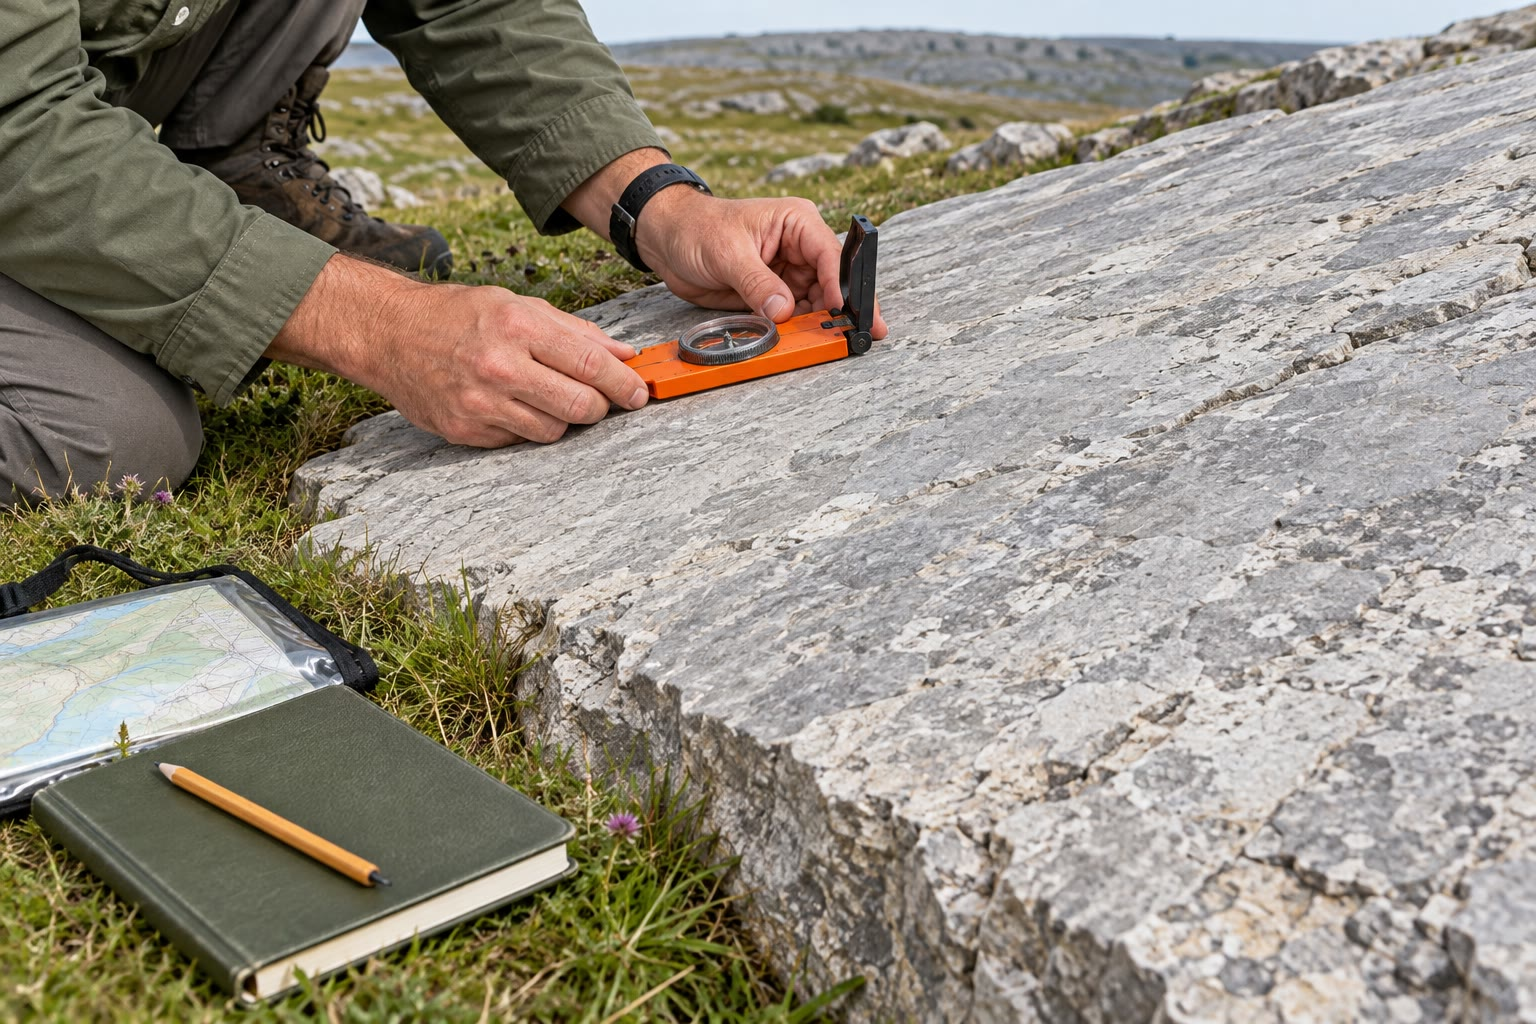
\includegraphics[width=0.6\linewidth]{images/book3/ai/b1-compass-clinometer.jpg}
\end{center}
\end{inthefield}

\begin{history}[第一幅国家地质图]
% ledger: gsl:smith-1815, commons:smith-1815
测量员威廉·史密斯曾在英格兰挖掘运河、排干土地，
他注意到每一岩层都含有其独有的化石，且化石的先后顺序
处处相同。他借助化石辨认岩层，
并沿这些岩层横贯全国，历时十五年以上。他绘制的地图，
题为\emph{A Delineation of the Strata of England and Wales, with part of
Scotland}，其日期为 1815 年 8 月 1 日，
被认为是第一幅覆盖整个国家的\omterm{def:b1:geological-maps:geological-map}{地质图}。
\begin{center}
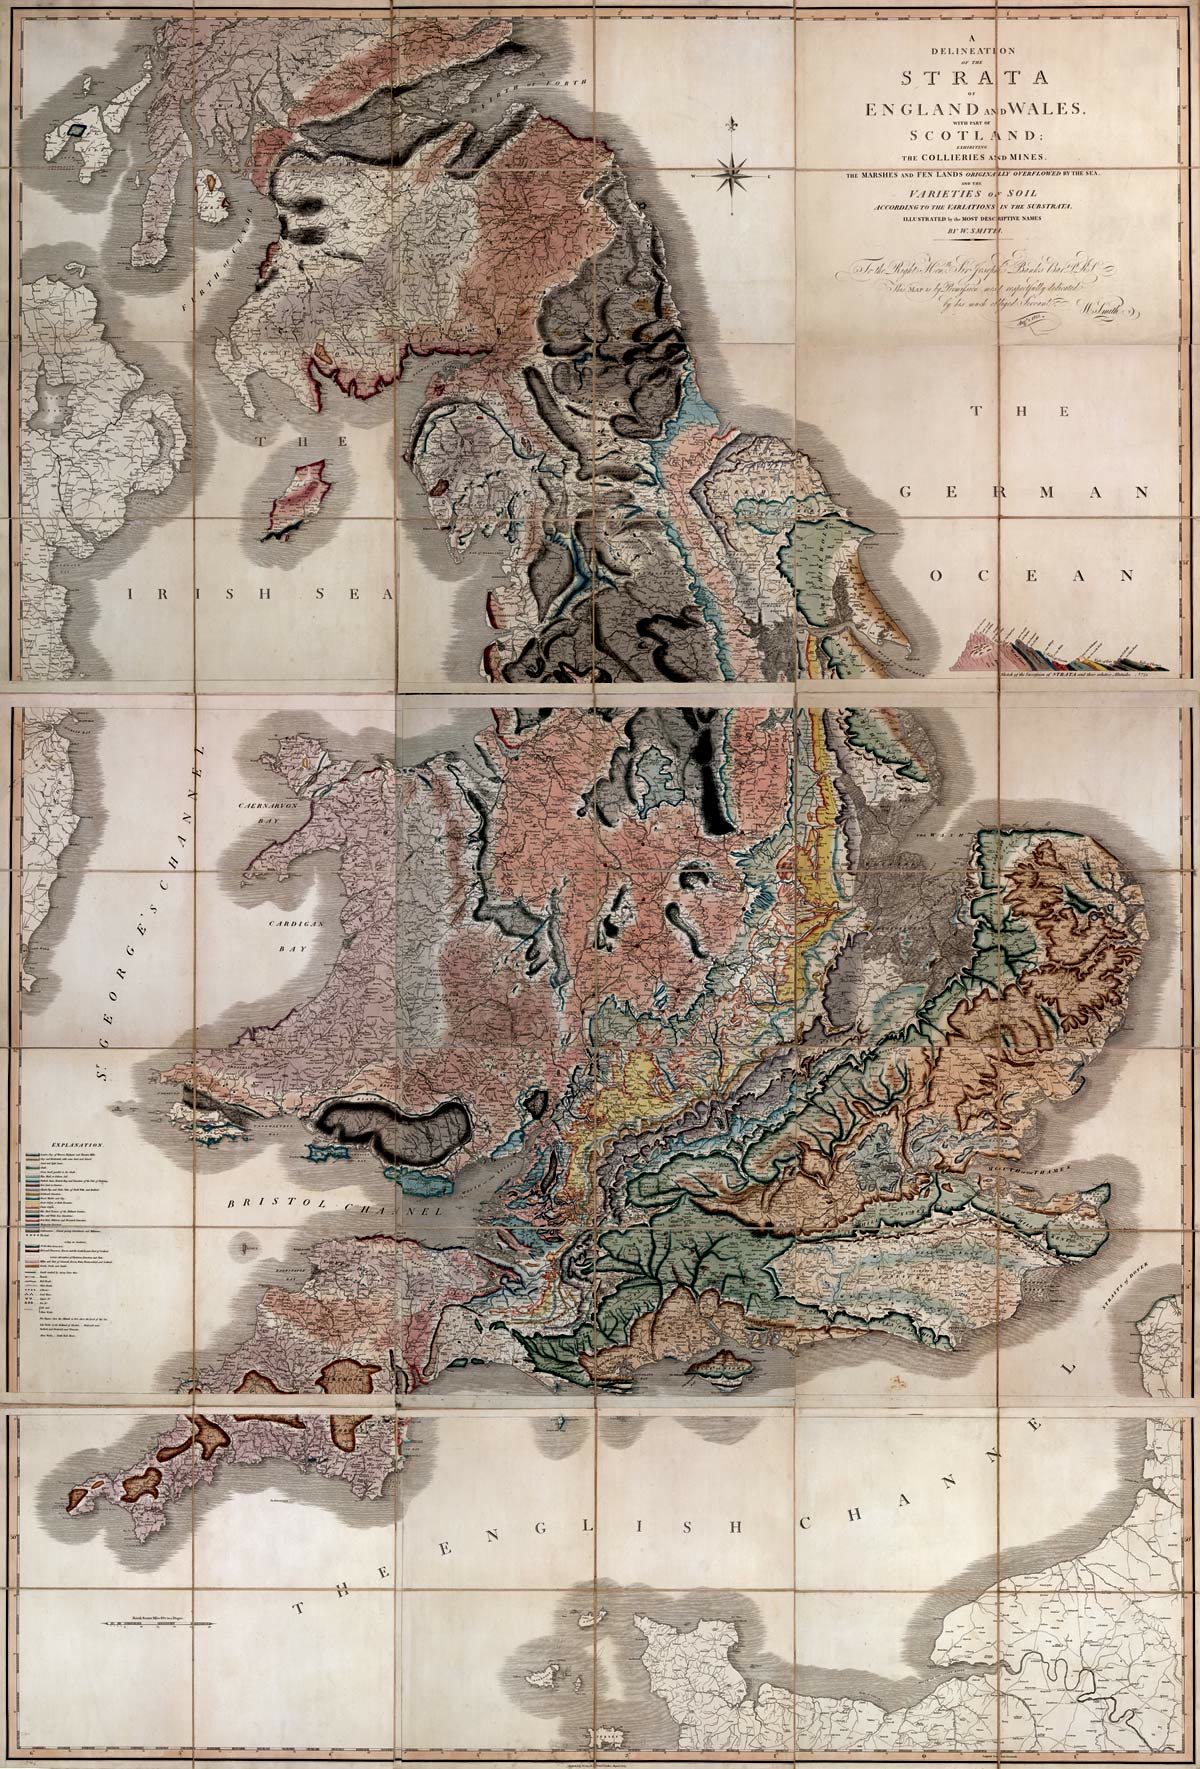
\includegraphics[width=0.36\linewidth]{images/book3/b1-smith-1815-map.jpg}

{\small 威廉·史密斯 1815 年的\omterm{def:b1:geological-maps:geological-map}{地质图}（公有领域）。}
\end{center}
\end{history}

\section{练习}

\begin{exercise}[$\star$]\label{exo:b1:geological-maps:1}
定义平面的\omterm{def:b1:geological-maps:attitude}{走向}、\omterm{def:b1:geological-maps:attitude}{倾角}和\omterm{def:b1:geological-maps:attitude}{倾向}。某岩层\omterm{def:b1:geological-maps:attitude}{产状}为
$135/40$，按右手定则给出其\omterm{def:b1:geological-maps:attitude}{走向}，并画出
其地图符号。
\end{exercise}

\begin{exercise}[$\star$]\label{exo:b1:geological-maps:2}
写出\omterm{def:b1:geological-maps:attitude}{产状}为 $090/30$、过点 $(0, 0, 500)$ 的平面方程，
坐标单位为米。该平面在 $(1000, 0)$ 和
$(0, 1000)$ 处的高程各为多少？
\end{exercise}

\begin{exercise}[$\star$]\label{exo:b1:geological-maps:3}
在地图上，某接触带的迹线恰好沿等高线 \qty{350}{m}
延伸，跨越数千米的丘陵与山谷。关于该接触带，能得出
什么结论？若其迹线是一条横穿丘陵和山谷的直线，
又当如何？
\end{exercise}

\begin{exercise}[$\star$]\label{exo:b1:geological-maps:4}
在瓦尔登丘陵的地图上，沿河流的\omterm{def:b1:geological-maps:fold}{背斜}核部
露出哪一单元，\omterm{def:b1:geological-maps:fold}{向斜}核部占据的是哪一单元？
试用叠加原理说明理由。
\end{exercise}

\begin{exercise}[$\star\star$]\label{exo:b1:geological-maps:5}
某接触带在高程 $\qty{300}{m}$ 处经过 $(0, 0)$，在高程 $\qty{300}{m}$
处经过 $(1000, 0)$，在高程 $\qty{200}{m}$ 处经过 $(0, 500)$（单位为米，$x$ 向东，$y$ 向北）。
先借助构造等高线推理，
再用\cref{thm:b1:geological-maps:three-point}，求其\omterm{def:b1:geological-maps:attitude}{走向}、\omterm{def:b1:geological-maps:attitude}{倾向}和\omterm{def:b1:geological-maps:attitude}{倾角}。
\end{exercise}

\begin{exercise}[$\star\star$]\label{exo:b1:geological-maps:6}
某河谷谷底向北以每千米 \qty{30}{m} 下降。若接触带分别为
(a) 水平；(b) 向南倾斜 \ang{20}；(c) 向北倾斜 \ang{1}；
(d) 向北倾斜 \ang{20}，则\omterm{def:b1:geological-maps:geological-map}{露头}的 V 字形尖端指向何方？请用
\cref{thm:b1:geological-maps:v-rule}加以论证。
\end{exercise}

\begin{exercise}[$\star\star$]\label{exo:b1:geological-maps:7}
在 V 字形法则的情形中，接触带以 $a = 0.364$
（\ang{20}）向下游倾斜，谷底以 $s = 0.03$ 下降。
谷坡上某点比谷底高 \qty{80}{m}。
该点处的迹线位于尖端上游多远？
\end{exercise}

\begin{exercise}[$\star\star$]\label{exo:b1:geological-maps:8}
瓦尔登\omterm{def:b1:geological-maps:fold}{背斜}的\omterm{def:b1:geological-maps:geological-map}{露头}在其核部北端处闭合。
\omterm{def:b1:geological-maps:fold}{褶皱轴}向哪个方向倾伏？\omterm{def:b1:geological-maps:fold}{向斜}的\omterm{def:b1:geological-maps:geological-map}{露头}
在靠近北端还是南端处闭合？
\end{exercise}

\begin{exercise}[$\star\star$]\label{exo:b1:geological-maps:9}
在\omterm{def:b1:geological-maps:geological-map}{地质图}上，沿断层看，地表哪一侧出露较新的单元？
哪一块下降了？请对照地图符号加以检验。
\end{exercise}

\begin{exercise}[$\star\star\star$]\label{exo:b1:geological-maps:10}
证明\omterm{def:b1:geological-maps:attitude}{产状}分别为 $(\alpha_1, \delta_1)$ 与
$(\alpha_2, \delta_2)$ 的两平面相交于一条与 $\vec n_1 \times \vec n_2$ 平行的直线，
其中 $\vec n_i = (\tan\delta_i\sin\alpha_i,
\tan\delta_i\cos\alpha_i, 1)$。将其应用于平面 $090/30$ 与 $270/30$：
该直线是什么？这两个平面构成何种\omterm{def:b1:geological-maps:fold}{褶皱}？
\end{exercise}

\begin{exercise}[$\star\star\star$]\label{exo:b1:geological-maps:11}
一垂直岩墙\omterm{def:b1:geological-maps:attitude}{走向}为 \ang{045}，在原点处于高程
\qty{0}{m} 的谷底出露。其迹线可能位于高程
\qty{300}{m} 的山丘何处？另一岩墙\omterm{def:b1:geological-maps:attitude}{走向}相同，
向东南倾斜 \ang{60}，同样在原点处出露。
在高程 \qty{300}{m} 的地面上，其迹线距原点多远、
位于何方向（沿垂直于\omterm{def:b1:geological-maps:attitude}{走向}的方向度量）？
\end{exercise}

\begin{exercise}[$\star\star\star$]\label{exo:b1:geological-maps:12}
在网格间距为 \qty{100}{m} 的\omterm{def:b1:geological-maps:dem}{数字高程模型}中，
$(x, y)$ 与 $(x + 100, y)$ 处的地面高程分别为 420 和 \qty{405}{m}，
$(x, y + 100)$ 处为 \qty{412}{m}。将该网格单元内的地面视为平面，
求其坡度（以度计）以及其朝向的\omterm{def:b1:spherical-astronomy:horizontal}{方位角}，
即下坡方向。
\end{exercise}

\section{问题：求解瓦尔登丘陵}

\begin{problem}[{周末问题——由钻孔与地图推断褶皱轴、
断层及该地区的历史}]
\label{pb:b1:geological-maps:1}
% all data computed in figdata/bachelor-1/varden_maps.py from the region's
% model (figdata/shared/region.py); invented region: exercise data, no ledger
某公司在瓦尔登丘陵钻探水井，记录了其钻孔与石灰岩底面
相遇的位置；其地质学家还确定了断层与地面相交的位置。
坐标以米计，自图幅西南角起算，向东、向北为正；
高程以米计，自海平面起算。第一部分使用
\cref{sec:b1:geological-maps:cut}中的彩色\omterm{def:b1:geological-maps:geological-map}{地质图}。

\medskip
\noindent\textbf{第一部分——读图。}
\begin{enumerate}
  \item 按从老到新的顺序列出该地区的各单元。
  \item 河流自西向东穿过哪些单元？
  \item 位于 $x = \qty{3.5}{km}$ 附近的\omterm{def:b1:geological-maps:fold}{褶皱}，其核部占据的是哪一单元？
        这是何种\omterm{def:b1:geological-maps:fold}{褶皱}？
  \item 位于 $x = \qty{7.5}{km}$ 附近的\omterm{def:b1:geological-maps:fold}{褶皱}，其核部占据的是哪一单元？
        这是何种\omterm{def:b1:geological-maps:fold}{褶皱}？
  \item 为何片岩与花岗岩仅在河流附近可见，
        即位于第一个\omterm{def:b1:geological-maps:fold}{褶皱}的核部？
  \item 砂岩与花岗岩之间是何种接触关系？
        请依据地图加以论证。
\end{enumerate}

\medskip
\noindent 钻孔（至石灰岩底面的深度 $d$，地面
高程 $z_g$），以及断层与基岩顶面相交的三个点 F1--F3
（F2 位于山谷中，处于较薄冲积层之下，该冲积层
未被断层切穿）：

\begin{omfigure}
\begin{minipage}[c]{0.42\linewidth}
\centering\small
\begin{tabular}{lrrrr}
\hline
 & 东 & 北 & $z_g$ & $d$ \\
\hline
E1 & 4000 & 6000 & 435 & 261 \\
E2 & 4600 & 7200 & 432 & 428 \\
E3 & 5100 & 6400 & 512 & 586 \\
W1 & 1500 & 6000 & 524 & 669 \\
W2 & 2200 & 7200 & 421 & 459 \\
W3 & 2600 & 5400 & 319 & 209 \\
\hline
 & 东 & 北 & $z_g$ & \\
\hline
F1 & 4197 & 1000 & 405 & \\
F2 & 5824 & 3500 & 129 & \\
F3 & 7321 & 6500 & 482 & \\
\hline
\end{tabular}
\end{minipage}\hfill
\begin{minipage}[c]{0.56\linewidth}
\centering
\begin{tikzpicture}
\begin{axis}[axis equal image, xmin=0, xmax=10, ymin=0, ymax=8, width=\linewidth,
  tick label style={font=\scriptsize}, xlabel={东 (km)}, ylabel={北 (km)},
  label style={font=\footnotesize}]
\addplot[fill=black!8, draw=black!50, line width=0.3pt, even odd rule] table {figdata/out/shared-region-unit-schist.dat};
\addplot[fill=black!8, draw=black!50, line width=0.3pt, even odd rule] table {figdata/out/shared-region-unit-granite.dat};
\addplot[fill=icsTriassic!20, draw=black!50, line width=0.3pt, even odd rule] table {figdata/out/shared-region-unit-sandstone.dat};
\addplot[fill=icsJurassic!25, draw=black!50, line width=0.3pt, even odd rule] table {figdata/out/shared-region-unit-limestone.dat};
\addplot[fill=icsJurassic!8, draw=black!50, line width=0.3pt, even odd rule] table {figdata/out/shared-region-unit-shale.dat};
\addplot[fill=icsCretaceous!20, draw=black!50, line width=0.3pt, even odd rule] table {figdata/out/shared-region-unit-chalk.dat};
\addplot[fault] table {figdata/out/shared-region-fault.dat};
\addplot[fill=omLithAlluv, draw=black!50, line width=0.3pt, even odd rule] table {figdata/out/shared-region-unit-alluvium.dat};
\addplot[river] table {figdata/out/shared-region-river.dat};
\addplot[only marks, mark=*, mark size=1.6pt] table[x=x_km, y=y_km] {figdata/out/bachelor-1-varden_maps-boreholes.dat};
\addplot[only marks, mark=square*, mark size=1.5pt, omThm] table[x=x_km, y=y_km] {figdata/out/bachelor-1-varden_maps-fault.dat};
\begin{scope}[every node/.style={font=\scriptsize\bfseries, inner sep=1.5pt, fill=white, fill opacity=0.8, text opacity=1}]
  \node[above right] at (axis cs:4,6) {E1};
  \node[above] at (axis cs:4.6,7.2) {E2};
  \node[right] at (axis cs:5.1,6.4) {E3};
  \node[above left] at (axis cs:1.5,6) {W1};
  \node[above] at (axis cs:2.2,7.2) {W2};
  \node[left] at (axis cs:2.6,5.4) {W3};
  \node[left, text=omThm] at (axis cs:4.197,1) {F1};
  \node[left, text=omThm] at (axis cs:5.824,3.5) {F2};
  \node[left, text=omThm] at (axis cs:7.321,6.5) {F3};
\end{scope}
\end{axis}
\end{tikzpicture}
\end{minipage}
\end{omfigure}

\medskip
\noindent\textbf{第二部分——东翼。}
\begin{enumerate}[resume]
  \item 计算 E1、E2 与 E3 处石灰岩底面的高程。
  \item 写出矢量 $\overrightarrow{E_1E_2}$ 与
        $\overrightarrow{E_1E_3}$。
  \item 计算二者的叉积，并使其朝上。
  \item 由此求出东翼石灰岩底面的\omterm{def:b1:geological-maps:attitude}{倾角}。
  \item 由此求出其\omterm{def:b1:geological-maps:attitude}{倾向}，再由右手定则求出\omterm{def:b1:geological-maps:attitude}{走向}。
  \item 所得结果是否与地图上东翼的
        \omterm{def:b1:geological-maps:attitude}{产状}符号相符？
\end{enumerate}

\medskip
\noindent\textbf{第三部分——\omterm{def:b1:geological-maps:fold}{褶皱}。}
\begin{enumerate}[resume]
  \item 计算 W1、W2 与
        W3 处石灰岩底面的高程。
  \item 求西翼上石灰岩底面的一个朝上法向量
        $\vec n_W$。
  \item 由此求西翼的\omterm{def:b1:geological-maps:attitude}{产状}。
  \item 求两翼交线（即\omterm{def:b1:geological-maps:fold}{褶皱轴}）的一个方向，
        即 $\vec n_E \times \vec n_W$（其中 $\vec n_E$ 取自第 9 题）。
  \item 给出\omterm{def:b1:geological-maps:fold}{褶皱轴}的倾伏向（轴线水平投影的\omterm{def:b1:spherical-astronomy:horizontal}{方位角}，
        沿下倾方向度量）与倾伏角（轴线
        与水平面的夹角）。
  \item 砂岩底面位于\omterm{def:b1:geological-maps:fold}{褶皱轴}上，河流穿过轴线处
        的高程为 \qty{230}{m}，位于 $y = \qty{4}{km}$ 附近。
        在轴线上向北 \qty{8}{km} 处，它要低多少？这与第一部分的
        第 3 题及\omterm{def:b1:geological-maps:geological-map}{露头}闭合性是否一致？
\end{enumerate}

\medskip
\noindent\textbf{第四部分——断层与历史。}
\begin{enumerate}[resume]
  \item 由 F1、F2 与 F3 求断层的\omterm{def:b1:geological-maps:attitude}{产状}。
  \item 沿断层，东南偏东一侧地表的单元
        比对侧的单元年轻。哪一盘下降？断层
        是正断层还是逆断层？
  \item 连接 F1 与 F3 的直线在 F2 以西约 \qty{200}{m} 处通过。
        为何断层迹线在河谷穿越处
        （即 F2 处）向东南偏东弯折？
  \item 按时间先后排列下列事件：\omterm{def:b1:geological-maps:fold}{褶皱}作用；白垩的沉积；断层作用；
        花岗岩的侵入；砂岩形成前的侵蚀；
        冲积层的沉积。
  \item 白垩为 9000 万年前形成，且已被\omterm{def:b1:geological-maps:fold}{褶皱}；冲积层
        沉积于最近 258 万年内，未被断层切割。
        \omterm{def:b1:geological-maps:fold}{褶皱}与断层作用分别发生在哪两个年龄之间？
  \item 若要钻至 F1 下方、海平面以下 \qty{1000}{m} 处的断层，
        竖直井应距 F1 多远、朝哪个方向钻？
\end{enumerate}
\end{problem}
